\documentclass[hyperref=unicode,presentation,10pt]{beamer}

\usepackage[absolute,overlay]{textpos}
\usepackage{array}
\usepackage{graphicx}
\usepackage{adjustbox}
\usepackage[version=4]{mhchem}
\usepackage{chemfig}
\usepackage{caption}
\usepackage{multirow}

%dělení slov
\usepackage{ragged2e}
\let\raggedright=\RaggedRight
%konec dělení slov

\addtobeamertemplate{frametitle}{
	\let\insertframetitle\insertsectionhead}{}
\addtobeamertemplate{frametitle}{
	\let\insertframesubtitle\insertsubsectionhead}{}

\makeatletter
\CheckCommand*\beamer@checkframetitle{\@ifnextchar\bgroup\beamer@inlineframetitle{}}
\renewcommand*\beamer@checkframetitle{\global\let\beamer@frametitle\relax\@ifnextchar\bgroup\beamer@inlineframetitle{}}
\makeatother
\setbeamercolor{section in toc}{fg=red}
\setbeamertemplate{section in toc shaded}[default][100]

\usepackage{fontspec}
\usepackage{unicode-math}

\usepackage{polyglossia}
\setdefaultlanguage{czech}

\def\uv#1{„#1“}

\mode<presentation>{\usetheme{default}}
\usecolortheme{crane}

\setbeamertemplate{footline}[frame number]

\usepackage{tikz}
\usetikzlibrary{positioning}
\usetikzlibrary{arrows}
\usetikzlibrary{shapes.multipart}

\title[Crisis]
{Hmotnostní spektrometrie}
\author
{Zdeněk Moravec, hugo@chemi.muni.cz}
\date{}

\titlegraphic{\includegraphics[keepaspectratio,width=5cm]{img/gcms-title.jpg}}

\begin{document}
\frame{\titlepage}

\section{Princip}
\frame{
	\frametitle{}
	\vfill
	\begin{itemize}
		\item Separační metoda.
		\item Principem hmotnostní spektrometrie je ionizace vzorku a analýza vzniklých iontů na základě jejich chování v magnetickém poli.
		\item Hmotnostní spektrum nejčastěji zobrazuje závislost intenzity signálu na poměru hmoty iontu a jeho náboje (\emph{m/z}).
	\end{itemize}
	\includegraphics[width=7cm]{img/acetone_ms.png}
	\vfill
}

\section{Stručná historie}
\frame{
	\frametitle{}
	\vfill
	\begin{itemize}
	\item \textbf{1912} První hmotnostní spektrometr, J.J. Thompson. První naměřená spektra \ce{O2}, \ce{N2}, \ce{CO2} a \ce{COCl2}.
	\item \textbf{1934} MS využita v organické chemii. R. Conrad
	\item \textbf{1940} Elektronová ionizace. C. Berry
	\item \textbf{1948} Publikován návrh nového analyzátoru typu TOF (Time Of Flight). A.E. Cameron, D.F. Eggers
	\item \textbf{1953} První kvadrupolární analyzátor, W. Paul a H. Steinwedel
	\item \textbf{1956} První spojení GC/MS. F.W. McLafferty, R.S. Gohlke
	\item \textbf{1966} Objev chemické ionizace. F. H. Field a M. S. B. Munson
	\item \textbf{1974} První spojení HPLC/MS. P.J. Arpino, M.A. Baldwin, F.W. McLafferty
	\item \textbf{1988} První použití ionizace elektrosprejem. J. Fenn
	\item \textbf{1999} Nový typ analyzátoru - Orbitrap. A.A. Makarov
	\end{itemize}
	\vfill
}

\section{Úvod do hmotnostní spektrometrie}
\subsection{Základní pojmy}
\frame{
	\frametitle{}
	\vfill
	\begin{itemize}
	\item Fragmentace - disociace nestabilních iontů vzniklých během ionizace analytu.
	\item Hmotnostní spektrum - závislost množství iontů na m/z.
	\item m/z - podíl hmotnosti iontu a jeho náboje.
	\item Molekulový pík - pík s hmotnostní odpovídající hmotnosti molekuly (M).
	\begin{itemize}
		\item M+1
		\item M+2
	\end{itemize}
	\item Základní pík - pík s nejvyšší intenzitou ve spektru.
	\end{itemize}
	\vfill
}

\subsection{Schéma hmotnostního spektrometru}
\frame{
	\frametitle{}
		\vfill
\begin{tikzpicture}
\draw [fill=white] (2,10) rectangle (0,9.5);
\node at (1,9.7) {Vzorek};

\draw [fill=white] (0,7.0) rectangle (2,8.5);
\node at (1,7.7) {Ionizátor};

\draw [fill=white] (7.2,4.5) rectangle (8.2,5.5);
\node at (7.7,5) {PC};

\draw [fill=white] (6.5,7) rectangle (8.8,8.5);
\node at (8.5,7.7) [text width = 3cm] {Detektor};


\draw [thick,<-, red] (6.5,7.75) -- (6,7.75);

\draw [fill=white] (3,7) rectangle (6,8.5);
\node at (4.5,7.7) {Analyzátor};

\draw [thick,<-, red] (3,7.75) -- (2,7.75);

\draw [thick,->, red] (7.7,7) -- (7.7,5.5);

\draw [thick,->, red] (1,9.5) -- (1,8.5);

\end{tikzpicture}
	\vfill
}

\section{Hmotnostní spektrometr}
\subsection{Iontový zdroj}
\frame{
	\frametitle{}
	\vfill
	\begin{itemize}
	\item \emph{Iontový zdroj} je odpovědný za ionizaci vzorku, která je nezbytá, aby mohla proběhnout jeho analýza. Podle množství dodané energie rozlišujeme měkké a tvrdé iontové zdroje.
	\item \emph{Elektronová ionizace (EI)} - iontový zdroj s tvrdou ionizací. Ionizace probíhá v plynné fázi, běžně se vyskytuje u sestav GC/MS. Principem je předávání energie letících elektronů analytu. Produktem je nejčastěji kladně nabitý radikál molekuly. Často dochází k rozsáhlé fragmentaci molekuly a ve spektru chybí molekulový pík.
	\item \emph{Chemická ionizace (CI)} - měkčí ionizace než EI. Nejprve ionizujeme reakční plyn (např. \ce{CH4}) a ten následně ionizuje molekuly analytu.
	\end{itemize}
	\vfill
}

\frame{
	\frametitle{}
	\vfill
	\begin{itemize}
	\item \emph{Elektrosprej (ESI)} - využívá se hlavně pro analýzu biologických vzorků. Ionizace probíhá působením silného elektrického pole (napětí 2-5 kV) na elektrodu. Ionizace probíhá za atmosférického tlaku.\footnote[frame]{Evan MAson, \href{https://commons.wikimedia.org/wiki/File\%3AElectrospray\_Ionization\_Spectroscopy.svg}{Electrospray Ionization Spectroscopy.svg}}
	\end{itemize}
	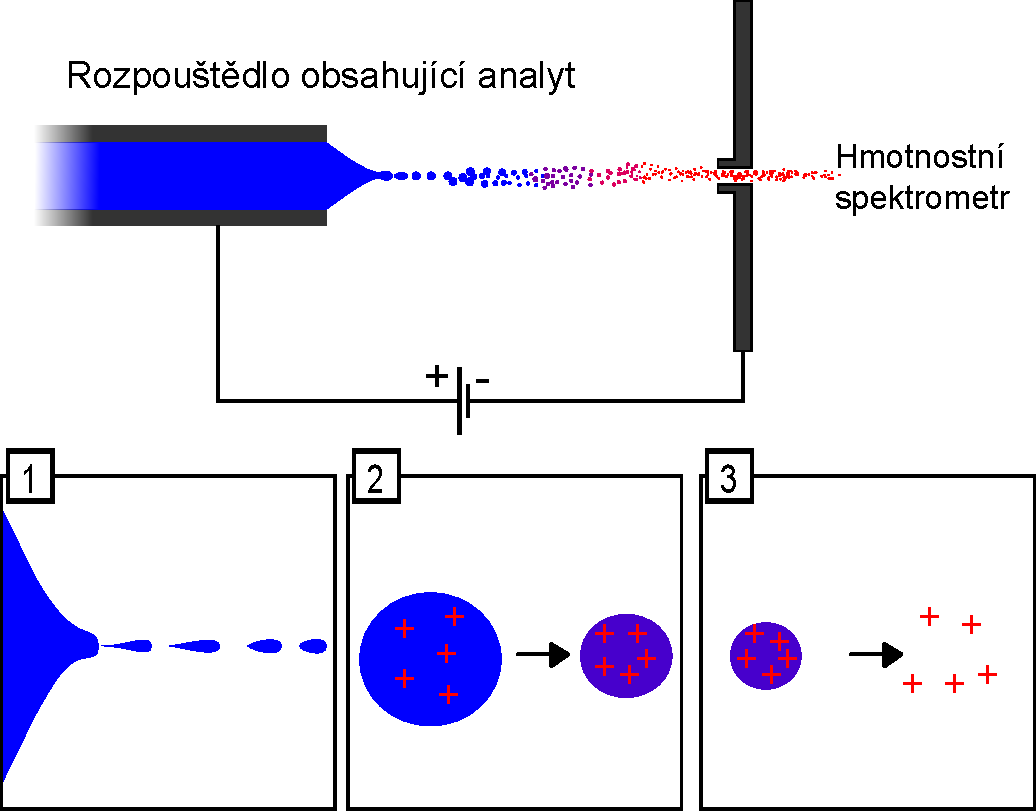
\includegraphics[width=6cm]{img/ESI.pdf}
	\vfill
}

\frame{
	\frametitle{}
	\vfill
	\begin{itemize}
	\item \emph{MALDI} - Matrix-Assisted Laser Desorption/Ionization
	\begin{itemize}
	\item Měkká ionizační technika. Využívá se při analýze biomolekul a~velkých organických molekul, které snadno fragmentují.
	\item Vzorek se nejprve smíchá s vhodnou matricí, např. kyselinou 2,5-dihydroxybenzoovou nebo 3,5-dimethoxy-4-hydroxyskořicovou a nanese se na kovové platíčko.
	\item Směs vzorku v matrici je ozářena pulsem laseru, čímž dojde k~ablaci a desorpci materiálu.
	\item Ionizace vzorku probíhá protonací matrice.
	\end{itemize}
	\end{itemize}
	\begin{center}
	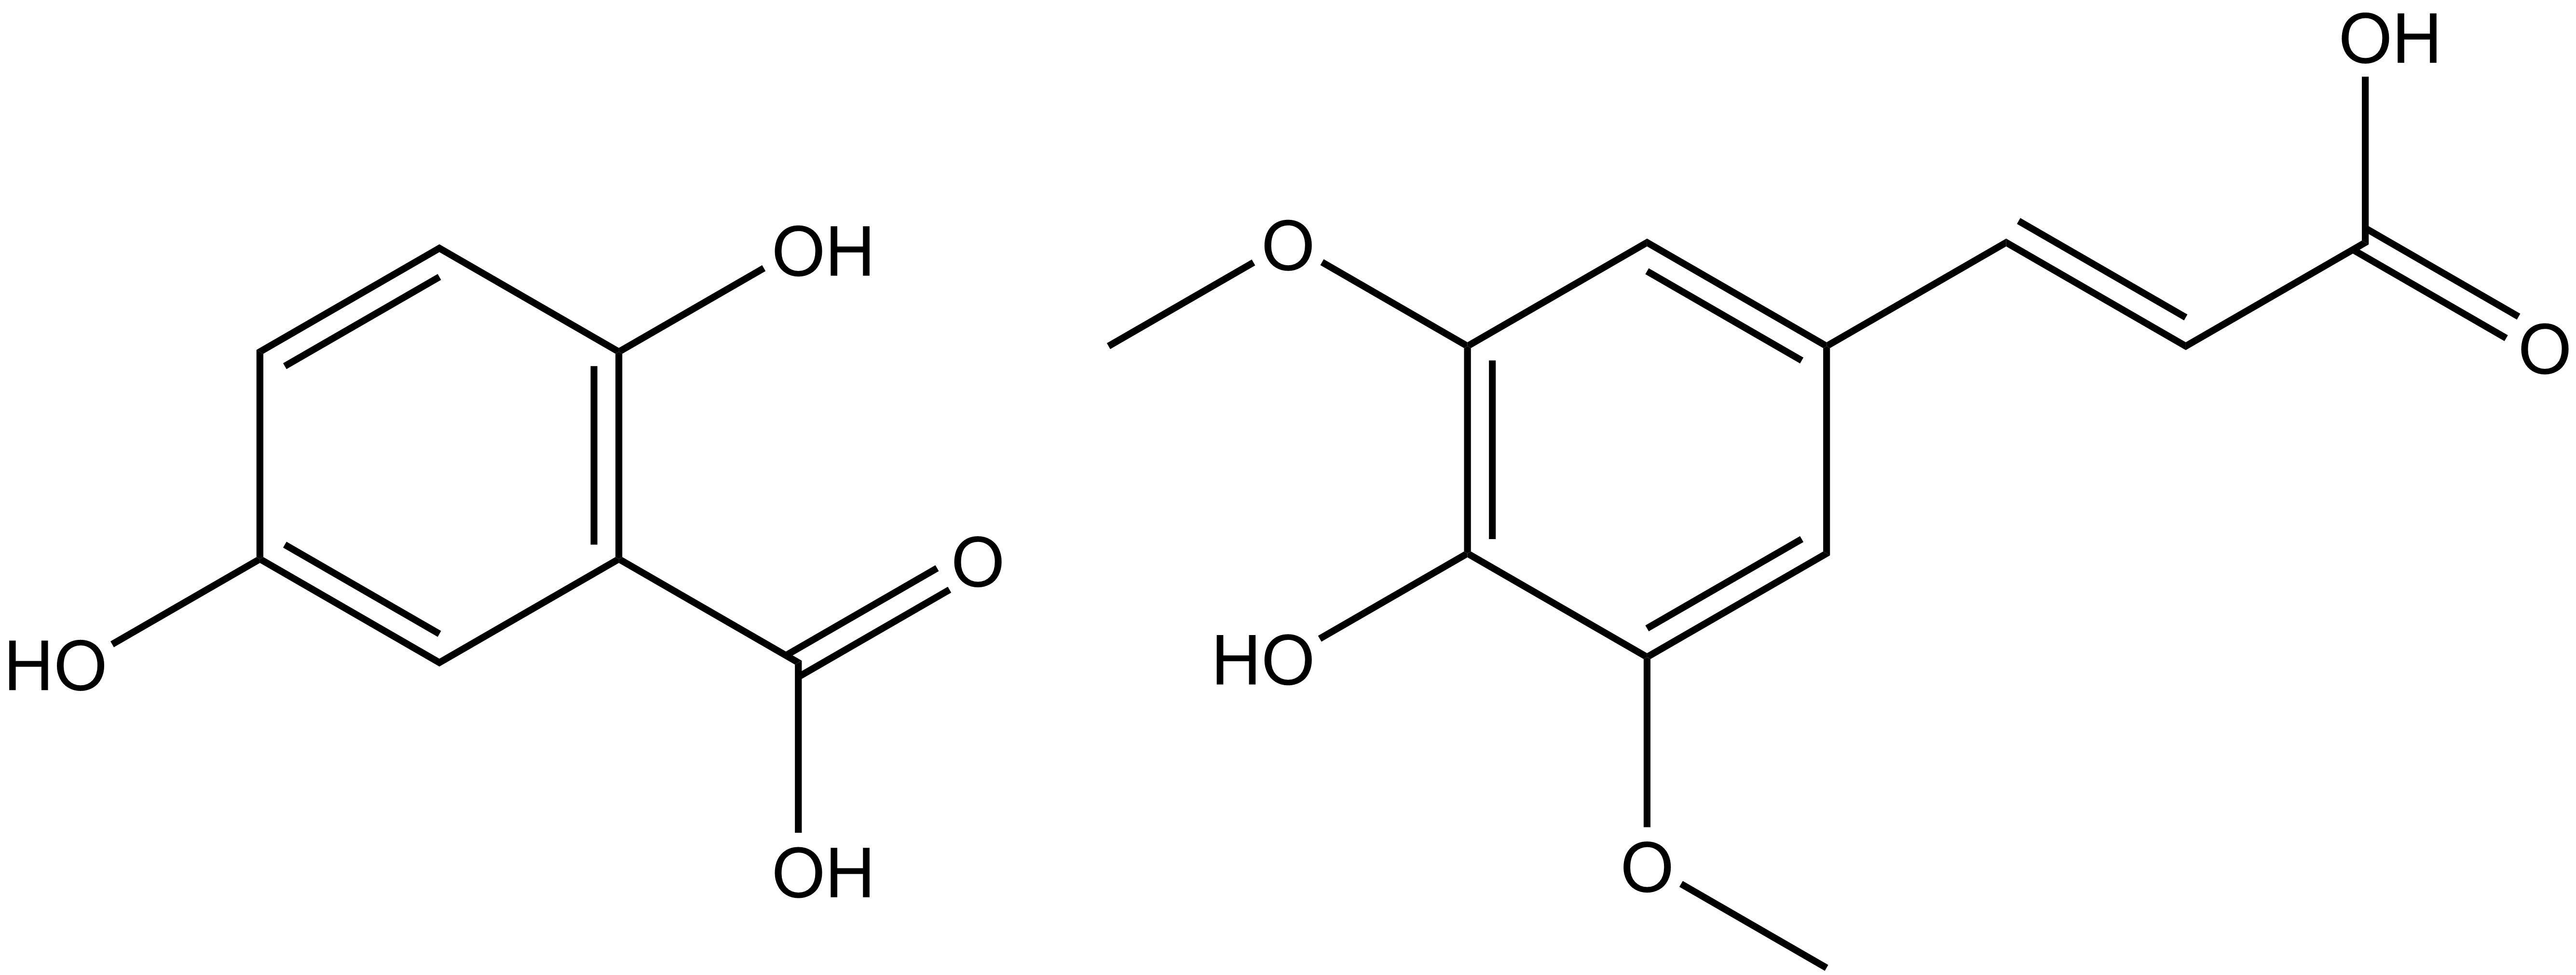
\includegraphics[width=\textwidth]{img/maldi-matrixes.png}
	\end{center}
	\vfill
}

\subsection{Analyzátor}
\frame{
	\frametitle{}
	\vfill
	\begin{itemize}
	\item \textit{Analyzátor} je součást MS spektrometru, kde dochází k separaci iontů podle poměru m/z.
	\item \emph{Kvadrupól} - nejběžnější a nejlevnější typ analyzátoru.
	\begin{itemize}
	\item Kombinace čtyř tyčí, na které je přivedeno stejnosměrné i~střídavé napětí. Úpravou velikosti stejnosměrného napětí a~amplitudy střídavého lze zvolit ionty s určitým poměrem m/z a~umožnit jim doputovat k detektoru, zatímco ostatní ionty jsou vychýleny mimo detektor.\footnote[frame]{Fulvio314, \href{https://commons.wikimedia.org/wiki/File:Mass\_spectrometer\_quadrupole.JPG}{Mass spectrometer quadrupole.JPG}}
	\item Analyzátor může pracovat buď jako skenovací, kdy postupně zvyšujeme hodnotu m/z nebo v režimu SIM (Single Ion Monitoring).
	\end{itemize}
	\end{itemize}
	\begin{center}
	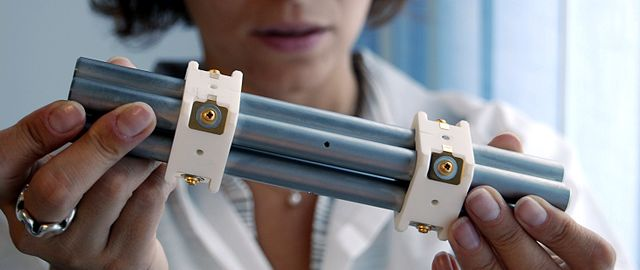
\includegraphics[width=4cm]{img/quadrupole.jpg}
	\end{center}
	\vfill
}

\frame{
	\frametitle{}
	\vfill
	\begin{columns}
	\column{.65\textwidth}
	\begin{itemize}
	\item \emph{Průletový analyzátor} - ionty jsou pulzně vpouštěny do evakuované trubice.\footnote[frame]{Mkotl, \href{https://commons.wikimedia.org/wiki/File:Time_Of_Flight_(TOF)_Mass_Analyser.gif}{Time Of Flight (TOF) Mass Analyser.gif}}
	\begin{itemize}
	\item Separace je založena na vztahu mezi dobou letu a hodnotou poměru m/z. Ionty s menším poměrem m/z proletí trubicí za kratší dobu.
	\item $\frac{m}{z} = \frac{2Vt^2}{l^2}$
	\item \textit{V - potenciál, t - doba letu iontu, l - délka trubice}
	\item Rozlišení analyzátoru lze zvýšit použitím iontového zrcadla (\textit{Reflektronu}) nebo tzv. opožděnou extrakcí, kdy dochází díky vzájemným srážkám iontů ke snížení rozdílů v kinetické energii iontů.
	\end{itemize}
	\end{itemize}
	\column{.3\textwidth}
	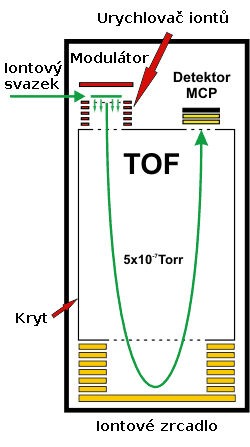
\includegraphics[width=4cm]{img/TOF.png}
	\end{columns}
	\vfill
}

\frame{
	\frametitle{}
	\vfill
	\begin{figure}
		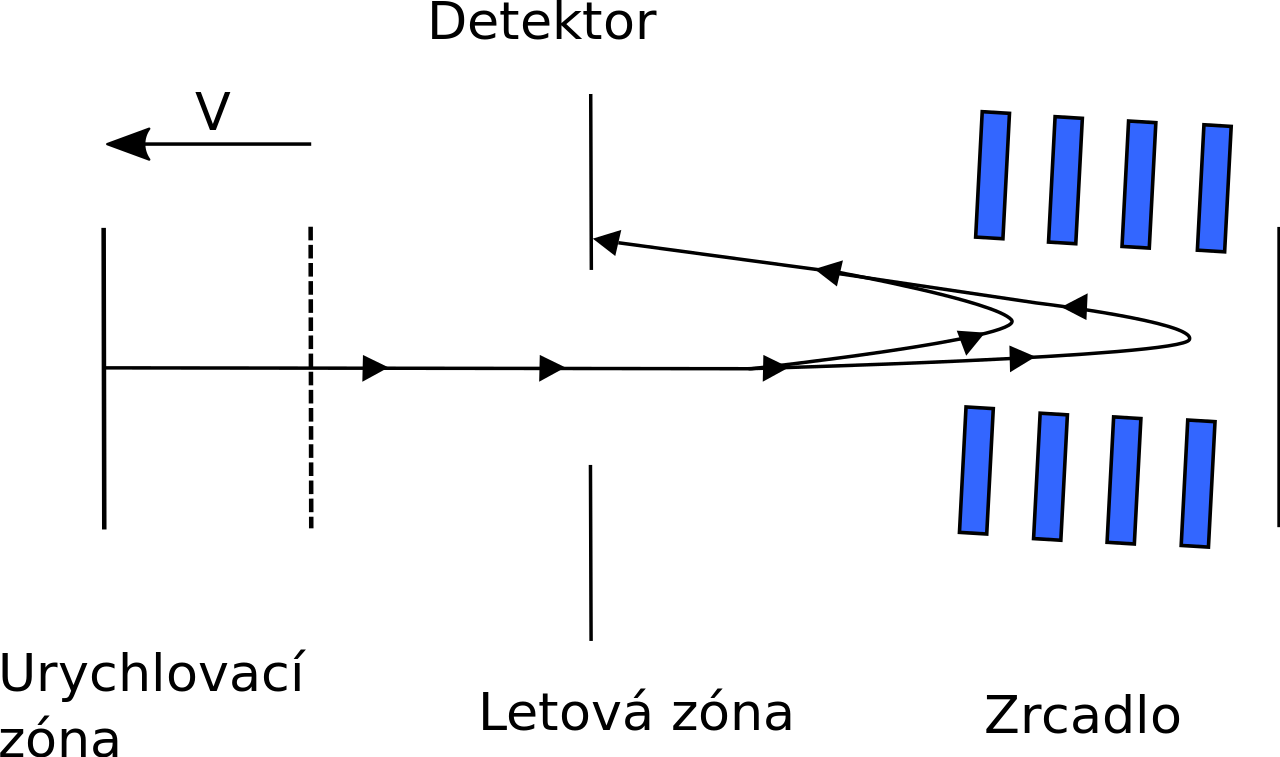
\includegraphics[height=.65\textheight]{img/TOF-Reflektor.png}
		\caption*{Schéma TOF analyzátoru s iontovým zrcadlem.\footnote[frame]{Zdroj: \href{https://commons.wikimedia.org/wiki/File:TOF-Reflektor.svg}{Elisemarion/Commons}}}
	\end{figure}
	\vfill
}

\frame{
	\frametitle{}
	\vfill
	\begin{figure}
		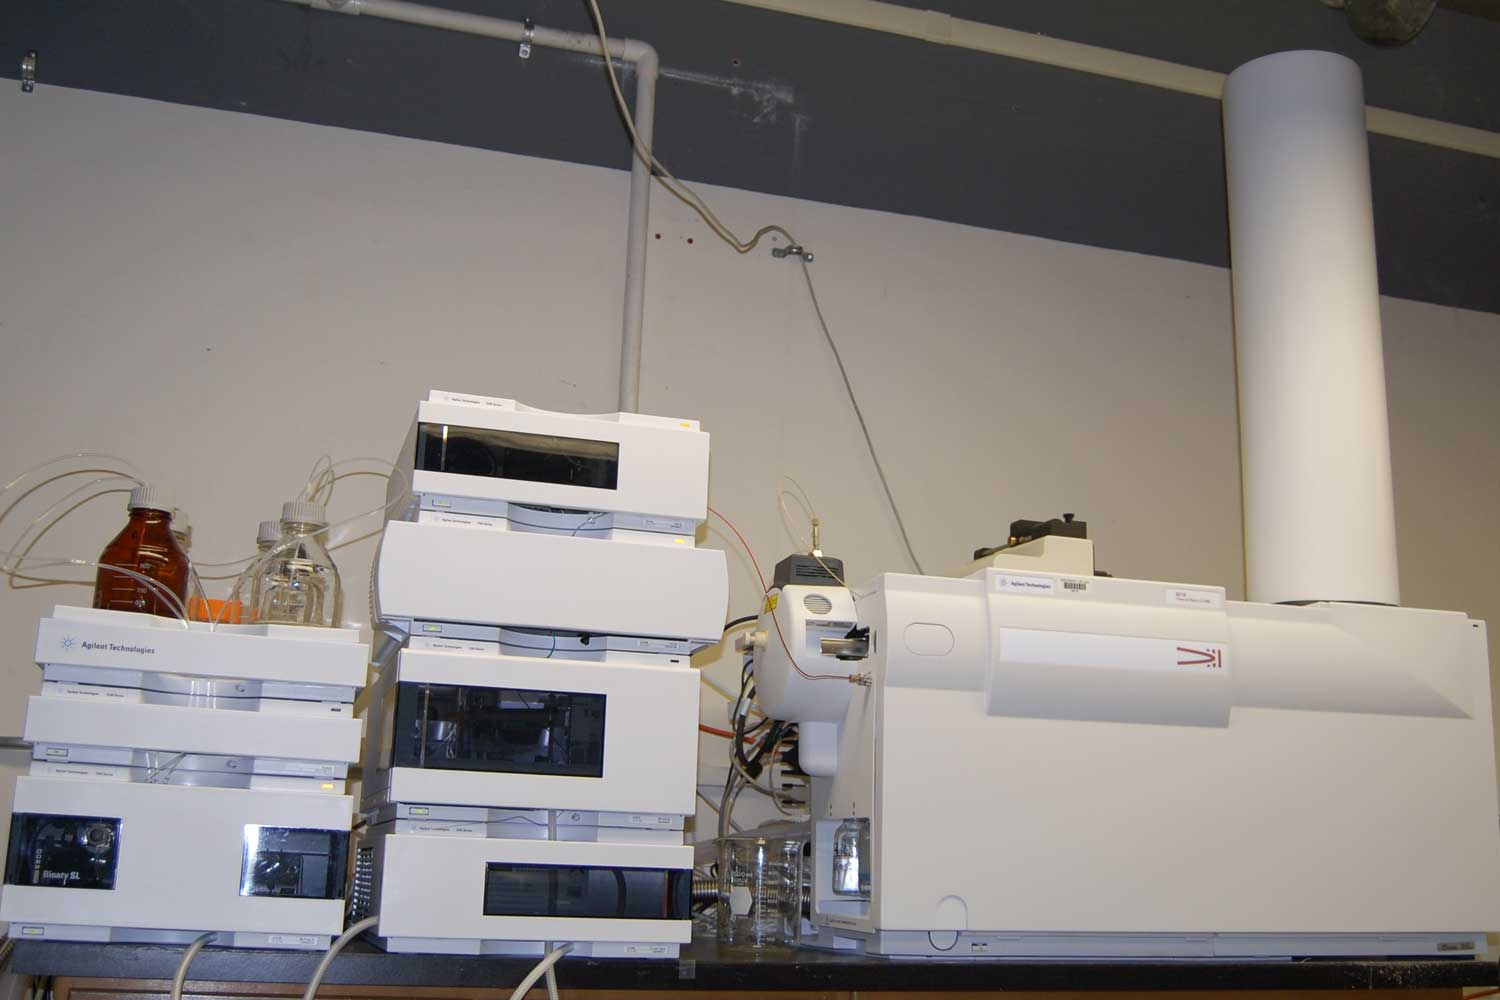
\includegraphics[height=.7\textheight]{img/ESI_TOF.jpg}
		\caption*{ESI-TOF MS spektrometr. TOF analyzátor je umístěn v kolmém směru.\footnote[frame]{Zdroj: \href{https://commons.wikimedia.org/wiki/File:ESI_TOF.jpg}{Kkmurray/Commons}}}
	\end{figure}
	\vfill
}

\frame{
	\frametitle{}
	\vfill
	\begin{itemize}
	\item \emph{Orbitrap} - elektrostatická orbitální past.\footnote[frame]{Thermo Fisher Scientific (Bremen), \href{https://commons.wikimedia.org/wiki/File:OrbitrapMA\%26Injector.png}{OrbitrapMA\&Injector.png}}
	\begin{itemize}
	\item Nejnovější typ hmotnostního analyzátoru.
	\item Skládá se z vnější a vřetenové elektrody, na které je přivedeno elektrické napětí.
	\item Ionty se pohybují okolo a podél středové elektrody.
	\item Frekvence v ose $z$ je nepřímo úměrná odmocnině z m/z.
	\item $\omega_z = \sqrt{\frac{k}{m/z}}$ [$\frac{rad}{s}$]
	\end{itemize}
	\end{itemize}
	\begin{center}
	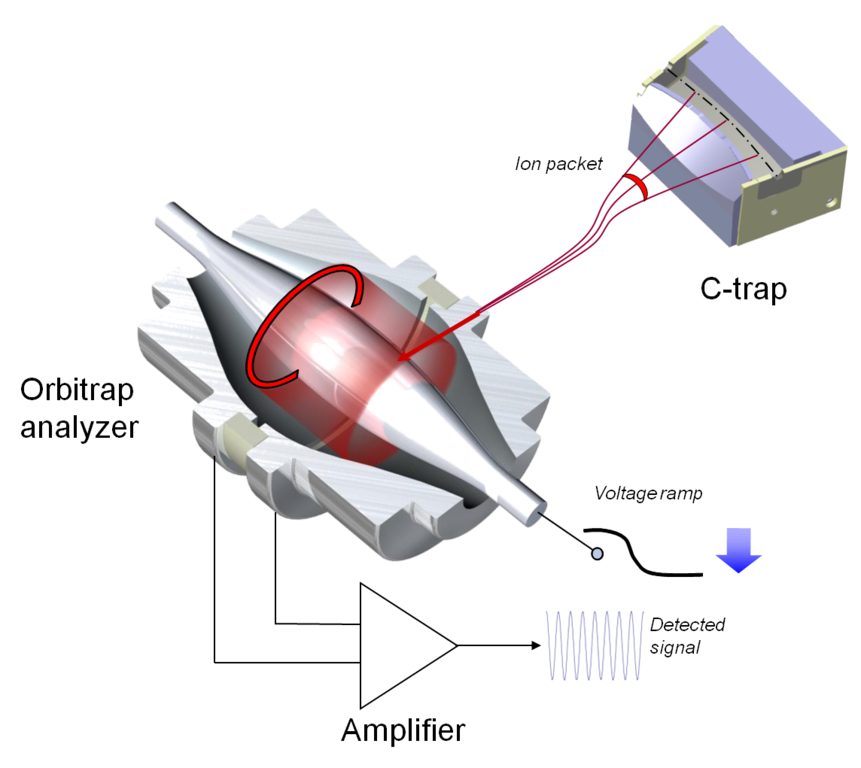
\includegraphics[height=3.9cm]{img/OrbitrapMA_Injector.png}
	\end{center}
	\vfill
}

\subsection{Detektor}
\frame{
	\frametitle{}
	\vfill
	\begin{itemize}
	\item Detektory dělíme na dvě skupiny:
	\begin{itemize}
		\item zaznamenávají všechny ionty, bez ohledu na jejich hodnotu m/z
		\item zaznamenávají ionty s ohledem na jejich hodnotu m/z
	\end{itemize}
	\end{itemize}

	\begin{figure}
		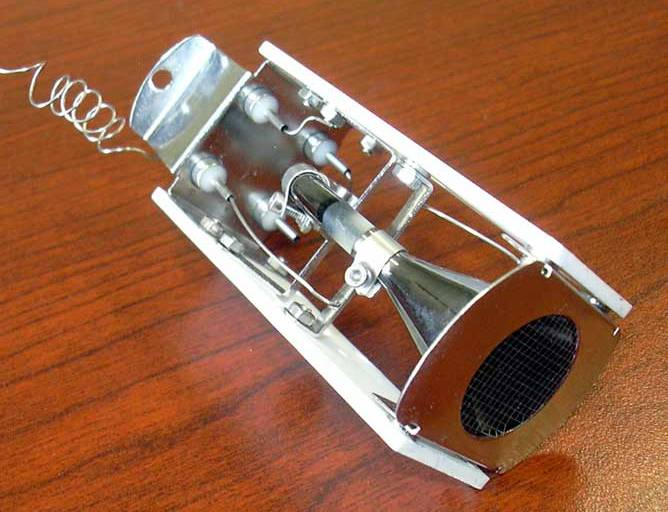
\includegraphics[height=.5\textheight]{img/Cont_dynode_detector.jpg}
		\caption*{Elektronový násobič.\footnote[frame]{Zdroj:  \href{https://commons.wikimedia.org/wiki/File:Cont_dynode_detector.jpg}{Kkmurray/Commons}}}
	\end{figure}
	\vfill
}


\frame{
	\frametitle{}
	\vfill
	\begin{itemize}
		\item \emph{Elektronový násobič} - letící iont vyrazí elektron z dynody násobiče, vyražený elektron putuje na další dynody a vyráží další elektrony. Detekce probíhá měřením vzniklého proudu.\footnote[frame]{\href{http://www.sge.com/products/electron-multipliers/how-electron-multipliers-work}{How Electron Multipliers work}}
	\end{itemize}
	\begin{figure}
		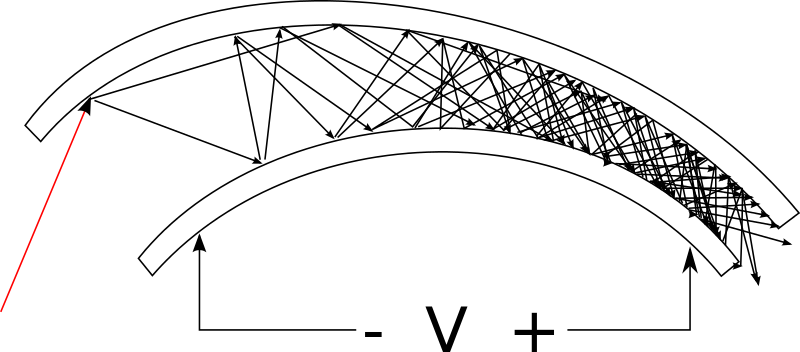
\includegraphics[height=3.8cm]{img/Electron_multiplier.png}
		\caption*{Princip funkce elektronového násobiče.\footnote[frame]{Zdroj:  \href{https://commons.wikimedia.org/wiki/File:Electron_multiplier.svg}{Egmason/Commons}}}
	\end{figure}
	\vfill
}

\section{Interpretace MS spekter}
\frame{
	\frametitle{}
	\vfill
	\begin{center}
	\includegraphics[height=8cm]{img/acetone_ms.png}
	\end{center}
	\vfill
}

\frame{
	\frametitle{}
	\vfill
	\begin{enumerate}
	\item Nalézt molekulový pík. Hledáme pík s nejvyšším poměrem m/z ve spektru.
	\item Pokusit se o vytvoření molekulového vzorce. Užitečnou pomůckou jsou píky izotopologů.
	\begin{itemize}
	\item \textit{Izotopology} jsou izomery se stejnou strukturou, ale lišící se izotopickým složením, např. \ce{CHCl3} a \ce{CDCl3}.
	\item Přírodní uhlík se skládá z izotopů $^{12}$C a $^{13}$C. Uhlíku $^{13}$C je 1,1 \%, tzn. že např. pro molekulu s pěti uhlíky bude intenzita píku M+1 rovna 6,6 \%.
	\item Interpretaci usnadňuje přítomnost píků M+2, pocházejících např. z O, Si, S, Cl, Br nebo I.
	\end{itemize}
	\item Pokud máme k dispozici databázi MS spekter, lze interpretaci zjednodušit a použít vyhledávácí algoritmus.
	\end{enumerate}
	\vfill
}

\subsection{Izotopové zastoupení běžných prvků}
\frame{
	\frametitle{}
	\vfill
	\begin{tabular}{|c|c|r@{,}l|c|r@{,}l|c|r@{,}l|}
	\hline
	\multirow{2}{*}{Prvek} & \multicolumn{3}{|c|}{M} & \multicolumn{3}{|c|}{M+1} & \multicolumn{3}{|c|}{M+2} \\
	& \multicolumn{1}{c}{m/z} &  \multicolumn{2}{c|}{\%} & \multicolumn{1}{c}{ m/z} & \multicolumn{2}{c|}{\%}
	& \multicolumn{1}{c}{ m/z} & \multicolumn{2}{c|}{\%} \\
	\hline
	H & 1 & 100 & 0 & 2 & 0 & 015 & \multicolumn{3}{c|}{} \\
	\hline
	C & 12 & 100 & 0 & 13 & 1 & 1 & \multicolumn{3}{c|}{} \\
	\hline
	N & 14 & 100 & 0 & 15 & 0 & 37 & \multicolumn{3}{c|}{} \\
	\hline
	O & 16 & 100 & 0 & 17 & 0 & 04 & 18 & 0 & 02 \\
	\hline
	F & 19 & 100 & 0 & \multicolumn{3}{c|}{} & \multicolumn{3}{c|}{} \\
	\hline
	Si & 28 & 100 & 0 & 29 & 5 & 1 & 30 & 3 & 4 \\
	\hline
	P & 31 & 100 & 0 & \multicolumn{3}{c|}{} & \multicolumn{3}{c|}{} \\
	\hline
	S & 32 & 100 & 0 & 33 & 0 & 79 & 34 & 4 & 4 \\
	\hline
	Cl & 35 & 100 & 0 & \multicolumn{3}{c|}{} & 34 & 32 & 0 \\
	\hline
	Br & 79 & 100 & 0 & \multicolumn{3}{c|}{} & 81 & 97 & 3 \\
	\hline
	I & 127 & 100 & 0 & \multicolumn{3}{c|}{} & \multicolumn{3}{c|}{} \\
	\hline
	\end{tabular}
	\vfill
}

\section{Využití MS spektroskopie}
\frame{
	\frametitle{}
	\vfill
	\begin{itemize}
	\item Farmacie
	\item Potravinářství
	\item Zemědělství
	\item Toxikologie
	\begin{itemize}
	\item Analýza léků
	\item Analýza metabolitů
	\end{itemize}
	\item Restaurování uměleckých předmětů
	\begin{itemize}
	\item Identifikace polymerů
	\item Identifikace přírodních látek - pryskyřic, lipidů, proteinů, apod.
	\item Datování předmětů pomocí $^{14}$C
	\end{itemize}
	\item Zjišťování izotopického složení - např. pro datování předmětů
	\item Vesmírný výzkum
	\item Preparativní MS - možnost syntézy látek s využitím MS
	\end{itemize}
	\vfill
}

\subsection{Analýza barviv a pryskyřic}
\frame{
	\frametitle{}
	\vfill
	Kombinace HPLC/MS.\footnote[frame]{SANTOS, Raquel, Jessica HALLETT, M. Conceição OLIVEIRA, Micaela M. SOUSA, Jorge SARRAGUÇA, M.S.J. SIMMONDS a M. NESBITT. HPLC-DAD-MS analysis of colorant and resinous components of lac-dye: A comparison between Kerria and Paratachardina genera. Dyes and Pigments [online]. 2015, 118, 129-136 [cit. 2019-11-22]. DOI: 10.1016/j.dyepig.2015.02.024.}
	\begin{center}
	\includegraphics[width=8cm]{img/MS-Example.png}
	\end{center}
	\vfill
}

\subsection{Analýza olejových barviv v dílech Edvarda Muncha}
\frame{
	\frametitle{}
	\vfill
	Kombinace LC/MS.\footnote[frame]{LA NASA, Jacopo, Marco ZANABONI, Daniele ULDANCK, et al. Novel application of liquid chromatography/mass spectrometry for the characterization of drying oils in art. Analytica Chimica Acta [online]. 2015, 896, 177-189 [cit. 2019-11-22]. DOI: 10.1016/j.aca.2015.09.023.}
	\begin{columns}
	\begin{column}{0.5\textwidth}
	\adjincludegraphics[width=3.6cm]{img/MS-Munch-paint.png}
	\end{column}

	\begin{column}{0.5\textwidth}
	\adjincludegraphics[width=4.3cm]{img/MS-Munch-MS.png}
	\end{column}

	\end{columns}
	\vfill
}

\section{Literatura}
\frame{
	\frametitle{}
	\vfill
	\begin{enumerate}
	\item DE HOFFMANN, Edmond a Vincent STROOBANT (ed.). \textit{Mass spectrometry: principles and applications.} 3rd ed. Chichester: John Wiley \& Sons, 2007, xii, 489 s. ISBN 9780470033111.
	\item Gross, J. H. \textit{Mass Spectrometry, A Textbook}, Second Edition, Springer-Verlag Berlin Heidelberg, Germany, 2011, ISBN: 978-3-642-10709-2
	\item HÜBSCHMANN, Hans-Joachim. \textit{Handbook of GC-MS: fundamentals and applications.} Third edition. Wiley-VCH Verlag GambH \& Co. KGaA, 2015, xvi, 863 stran. ISBN 978-3-527-33474-2.
	\end{enumerate}
	\vfill
}

\end{document}
